\begin{frame}{$d(K^-, n K^0)"n"$ イベント}
  \tminipageTwo{
    \begin{figure}
      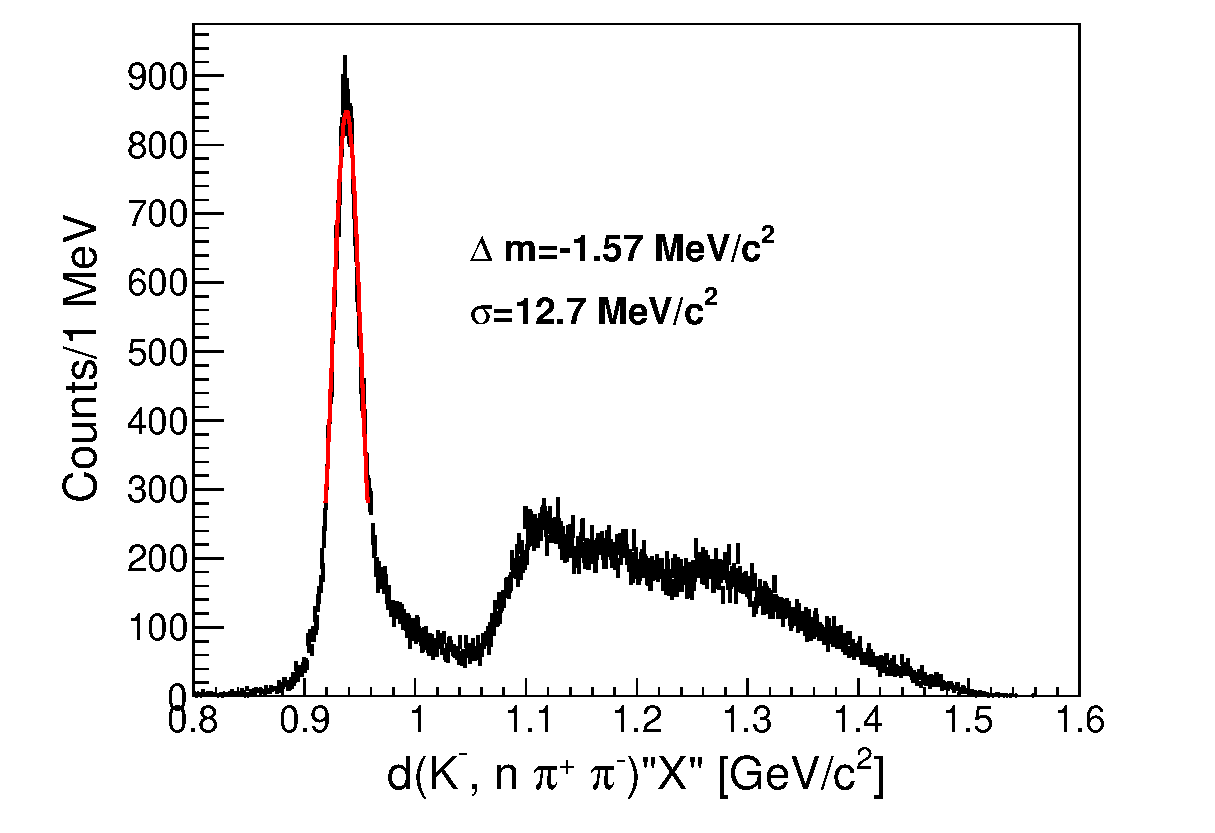
\includegraphics[width=3cm]{../pic/Run78/KN_ana_NC170_2sigma/KNpipi_MM_woFit.eps}
      \captionsetup{font=scriptsize}
      \caption{
        $d(K^-, n \pi^+ \pi^-)"n"$のイベント選別
      }
    \end{figure}
  }{
    \begin{figure} 
      \includegraphics[width=3cm]{../pic/Run78/KN_ana_NC170_2sigma/IM_pipi_select.eps}
      \captionsetup{font=scriptsize}
      \caption{
        \centering
        $K^0$の選別、色線はp.\pageref{page:Fit_IM}のフィットで見積もられた。
        バックグランドのイベントの分布を表す。
      }
    \end{figure}
  }
  \begin{tabular}{cc}
    \begin{minipage}{0.4\hsize}
      \begin{figure}
        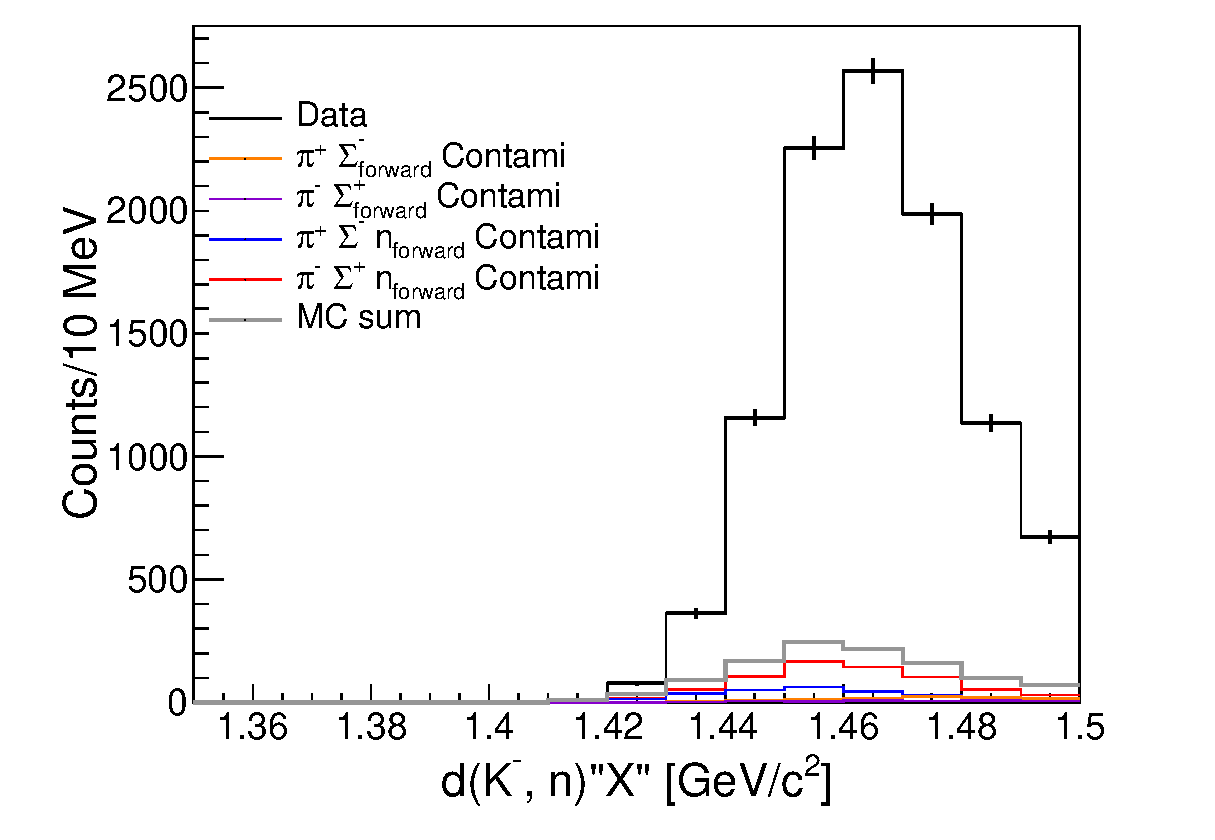
\includegraphics[width=5cm]{../pic/Run78/QE/KN_MM_wK0_tag.eps}
      \end{figure}
    \end{minipage}
    \begin{minipage}{0.6\hsize}
      \centering
      \scriptsize
      左図は上右図によって$K^0$選別されたイベント\\
      色線は他の反応からのバックグラウンド
    \end{minipage}
  \end{tabular}
\end{frame}
